
The given  equations can be expressed as the matrix equation
\begin{align}
     \myvec{\frac{3}{2}&\frac{5}{3}\\9&-10}\vec{x}=\myvec{7\\14}
\end{align}
The augmented matrix  is row reduced as
\begin{align}
     \myvec{\frac{3}{2}&\frac{5}{3}& 7\\
           9 & -10 & 14}
          \xleftrightarrow{R_1 \leftarrow\frac{2}{3}{R_1}}
    \myvec{1&\frac{10}{9}&\frac{14}{3}\\
        9&-10&14}\\
        \xleftrightarrow{R_2\leftarrow R_2 -9R_1}
    \myvec{1&\frac{10}{9}&\frac{14}{3}\\0&-20&-28}\\
    \xleftrightarrow{R_2\leftarrow \frac{-1}{20}{R_2}}
    \myvec{1&\frac{10}{9}&\frac{14}{3}\\0&1&\frac{7}{5}}\\
    \xleftrightarrow{R_1\leftarrow \frac{-10}{9}R_2+R_1}
    \myvec{1&0&\frac{28}{9}\\0&1&\frac{7}{5}}
    \end{align}
   $\therefore$ the given system is consistent as can be verified from Fig. \ref{2/5/cFig:Graphical Solution}
\begin{figure}[!ht]
    \centering
    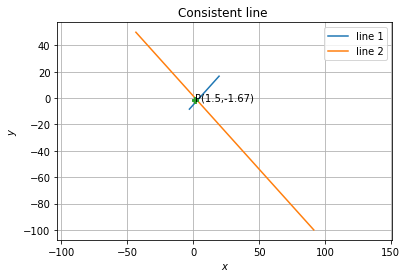
\includegraphics[width= \columnwidth]{solutions/sep/2/5/c/consistent line.png}
    \caption{Graphical solution}
    \label{2/5/cFig:Graphical Solution}
\end{figure}
  